\subsection{Method of Maximum Likelihood}
\label{subsec:method-of-maximum-likelihood}

Since the sample $\boldsymbol{X} = (X_1,\ \ldots,\ X_n)$ has already been observed, we find such parameters that maximize the probability (likelihood) for this to happen. In other words, we make the event that has already happened to be as likely as possible. This is yet another way to make the chosen distribution consistent with the observed data.
\begin{definition}{}
  \textbf{Maximum likelihood estimator} is the parameter value that maximizes the likelihood of the observed sample.
  \begin{itemize}
    \item For a discrete distribution, we maximize the joint pmf of data $P(X_1,\ \ldots,\ X_n)$.
    \item For a continuous distribution, we maximize the joint density $f(X_1,\ \ldots,\ X_n)$.
  \end{itemize}
\end{definition}

\subsubsection{Discrete Case}
\label{subsubsec:disc-case}

For a discrete distribution, the probability of a given sample is the joint pmf of data,
\begin{align*}
  \prob{\boldsymbol{X} = (X_1,\ \ldots,\ X_n)} = P(\boldsymbol{X}) &= P(X_1,\ \ldots,\ X_n) \\
  &= \prod_{i=1}^{n} P(X_i)
\end{align*}
because in a simple random sample, all observed $X_i$ are independent.

To maximize this likelihood, we consider the critical points by taking derivatives with respect to all unknown parameters and equating them to 0.  The maximum can only be attained at such parameter values $\theta$ where the derivative $\frac{\partial}{\partial\theta} P(X)$ equals 0, where it does not exist, or at the boundary of the set of possible values of $\theta$.

A nice computational shortcut is to take logarithms first. Differentiating the sum
\begin{equation*}
  \ln \prod_{i=1}^{n} P(X_i) = \sum_{i=1}^{n} \ln P(X_i)
\end{equation*}
is easier than differentiating the product $\prod P(X_i)$. Besides, logarithm is an increasing function, so the likelihood $P(\boldsymbol{X})$ and the log-likelihood $\ln P(\boldsymbol{X})$ are maximized by exactly the same parameters.

\textbf{\textit{Check the example 9.7 from textbook.}}

\subsubsection{Continuous Case}
\label{subsubsec:cont-case}

In the continuous case, the probability to observe exactly the given number $X = x$ is $0$. Instead, the method of maximum likelihood will maximize the
probability of observing ``almost'' the same number.

For a very small $h$,
\begin{equation*}
  \prob{x - h < X < x + h} = \int_{x - h}^{x + h} f(y) d(y) \approx (2h) f(x)
\end{equation*}
That is, the probability of observing a value close to $x$ is proportional to the density $f(x)$ (see Figure 1). Then, for a sample $\bs{X} = (X_1,\ \ldots,\ X_n)$, the maximum likelihood method will maximize the joint density $f(X_1,\ \ldots,\ X_n)$.
\begin{figure}[H]
  \centering
  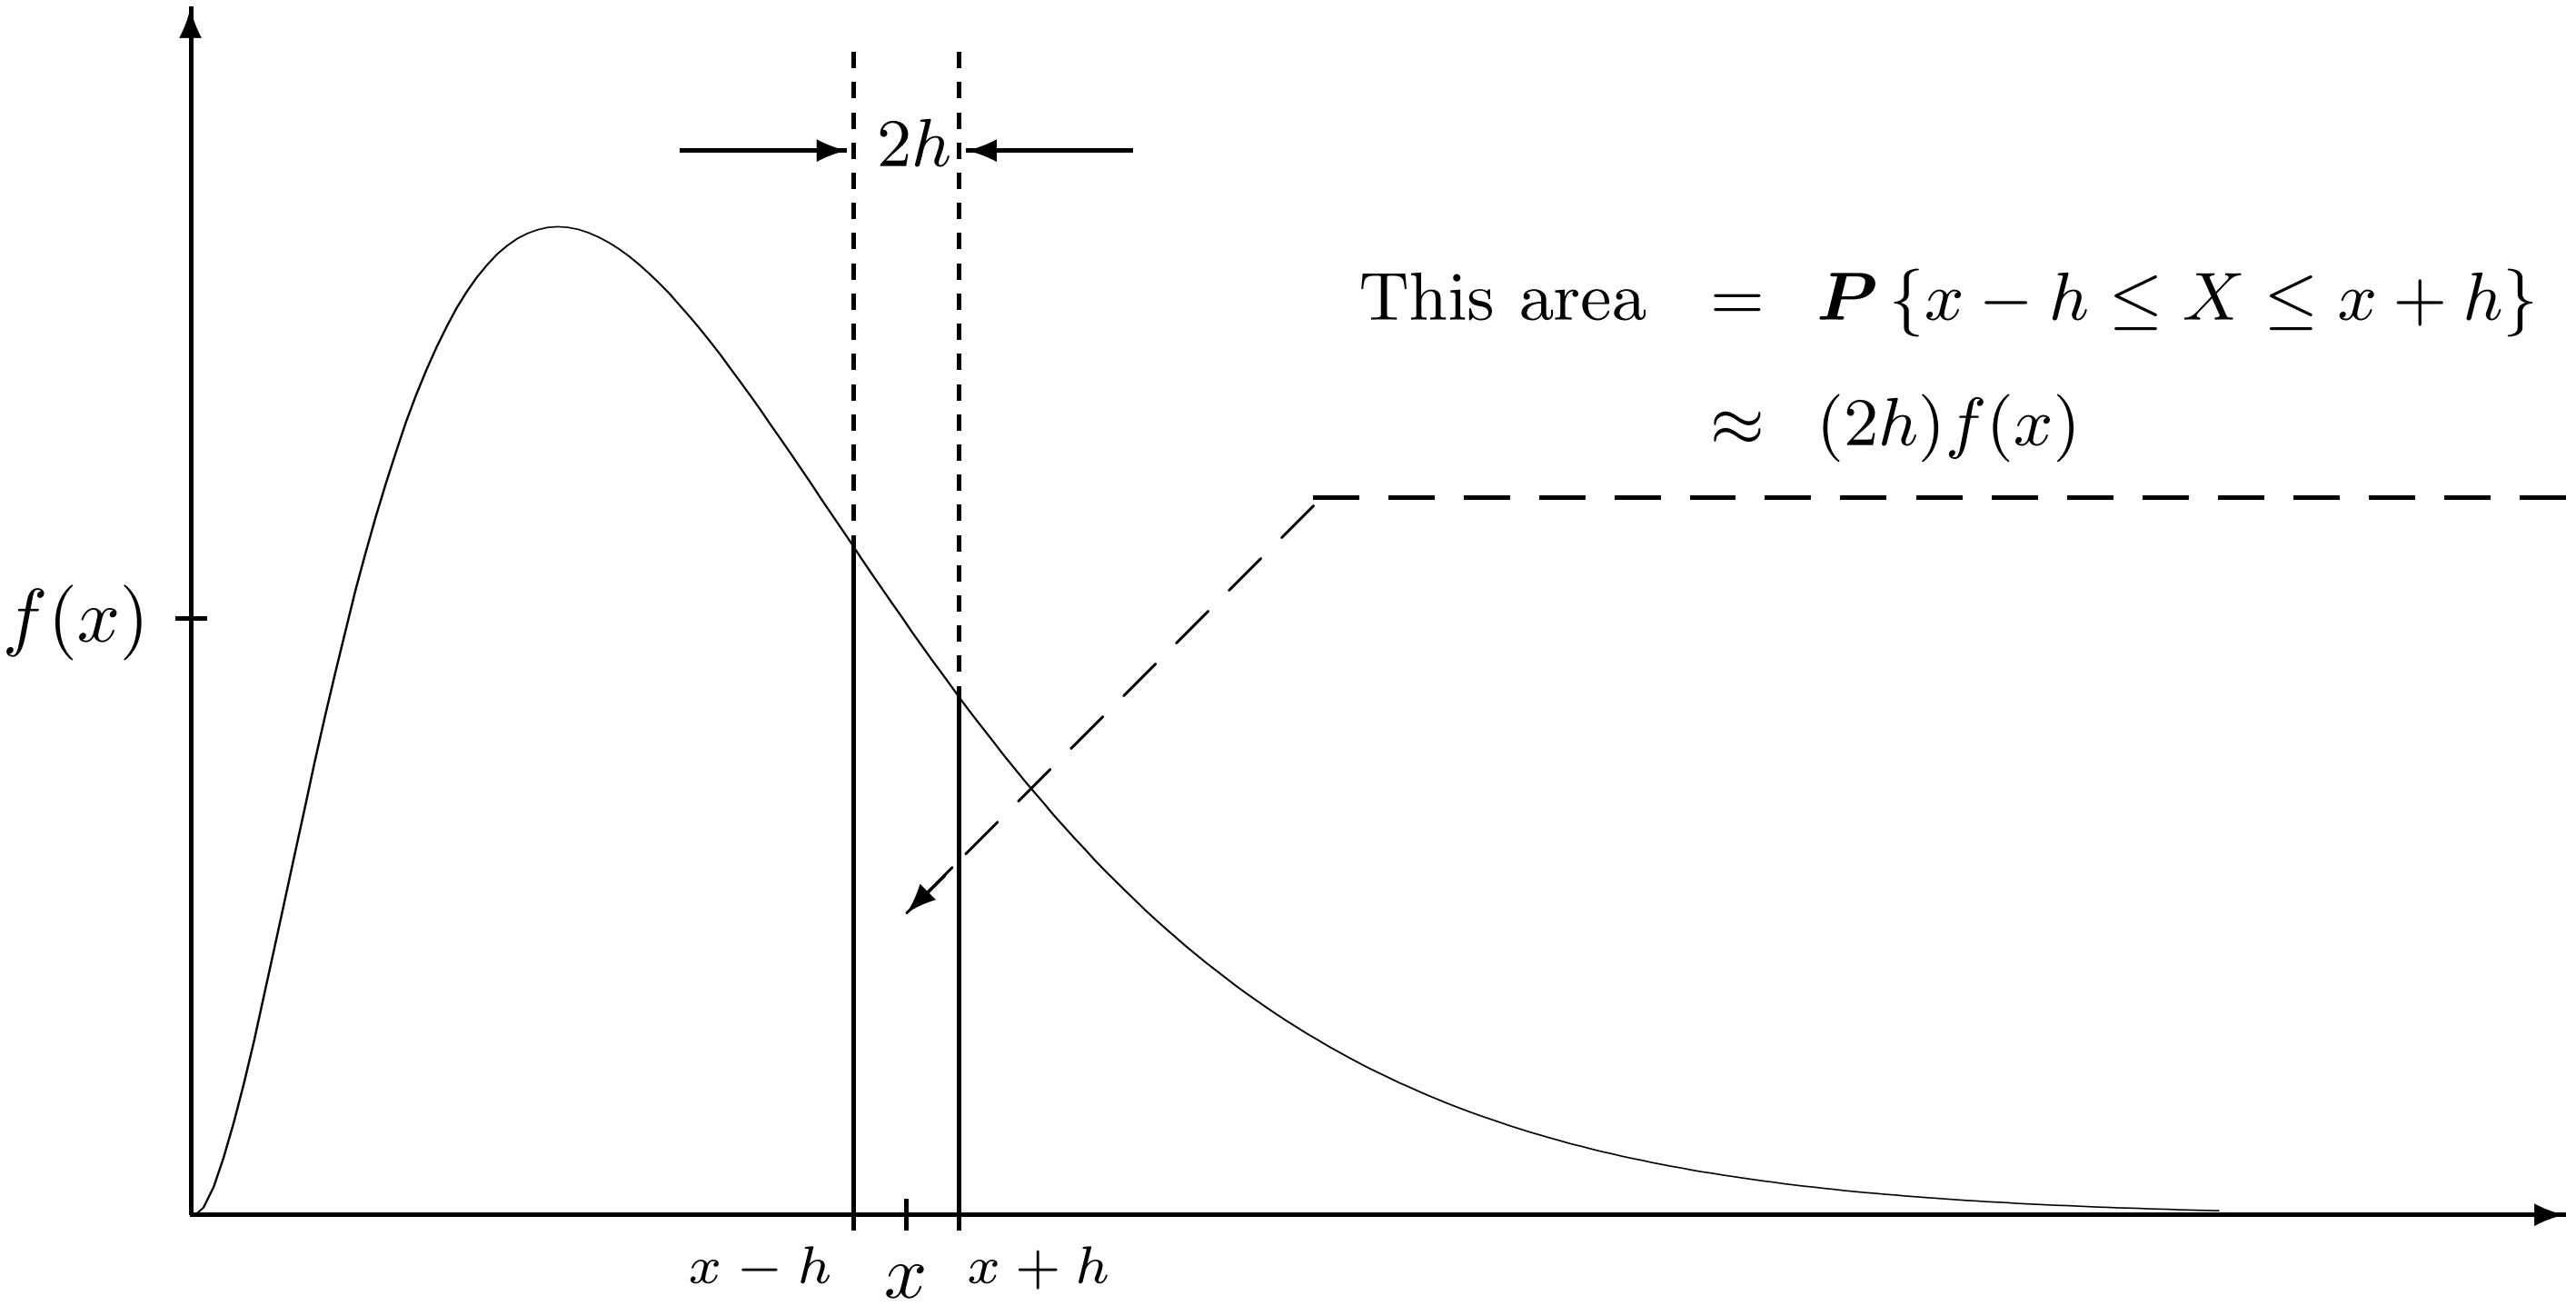
\includegraphics[width=\linewidth]{img/fig-9.1.png}
  \caption{}
  \label{fig:9.1}
\end{figure}

\textbf{\textit{Check the examples 9.8 and 9.9 from textbook.}}

Sometimes the likelihood has no critical points inside its domain, then it is maximized at the boundary.

When we estimate more than $1$ parameter, all the partial derivatives should be equal $0$ at the critical point. If no critical points exist, the likelihood is again maximized on the boundary.

Maximum likelihood estimators are rather popular because of their nice properties. Under mild conditions, these estimators are consistent, and for large samples, they have an approximately Normal distribution. Often in complicated problems, finding a good estimation scheme may be challenging whereas the maximum likelihood method always gives a reasonable solution.

\vspace*{\fill}
\columnbreak
